\chapter{Cause-specific mortality rates: alcohol dependence}
\label{applications-csmr}

A key assumption of the YLL estimates in the GBD 2010 Study is that only
one cause leads to death.  This categorical attribution of deaths in
a mutually exclusive way has the desirable property that all assigned
deaths sum to the total number of deaths.  However, this
creates a rate that does not directly correspond to any rate in the
compartmental model (figure~\ref{forward-sim-two-compartment}) because it
assumes that all who die \emph{with} the condition die \emph{of} the
condition.  While this is a reasonable assumption for conditions
such as cancer, cirrhosis, or diarrhea, it is not for conditions such as
alcohol dependence, where many people die \emph{with}
the condition but \emph{not of} it.  Using alcohol dependence as an
example, this chapter compares the results of
the modeling assumptions of those who die \emph{of} alcohol dependence
and those who die \emph{with} alcohol dependence but from other causes.

Alcohol dependence is the dysfunctional pattern of alcohol consumption
that leads to physiological dependence and impaired control.  Similar to
cocaine dependence (chapter~\ref{applications-splines_knot_loc}), in order to
be diagnosed with alcohol dependence, $3$ or more of the $7$
substance dependence criteria identified by the American Psychiatric
Association must be
fulfilled within a $12$-month period.
\cite{american_psychiatric_association_diagnostic_2000, hasin_prevalence_2007}
Systematic review yielded prevalence, excess mortality, and
cause-specific mortality data as seen in figure~\ref{fig:app-alcohol
  data}.

    \begin{figure}[h]
        \begin{center}
            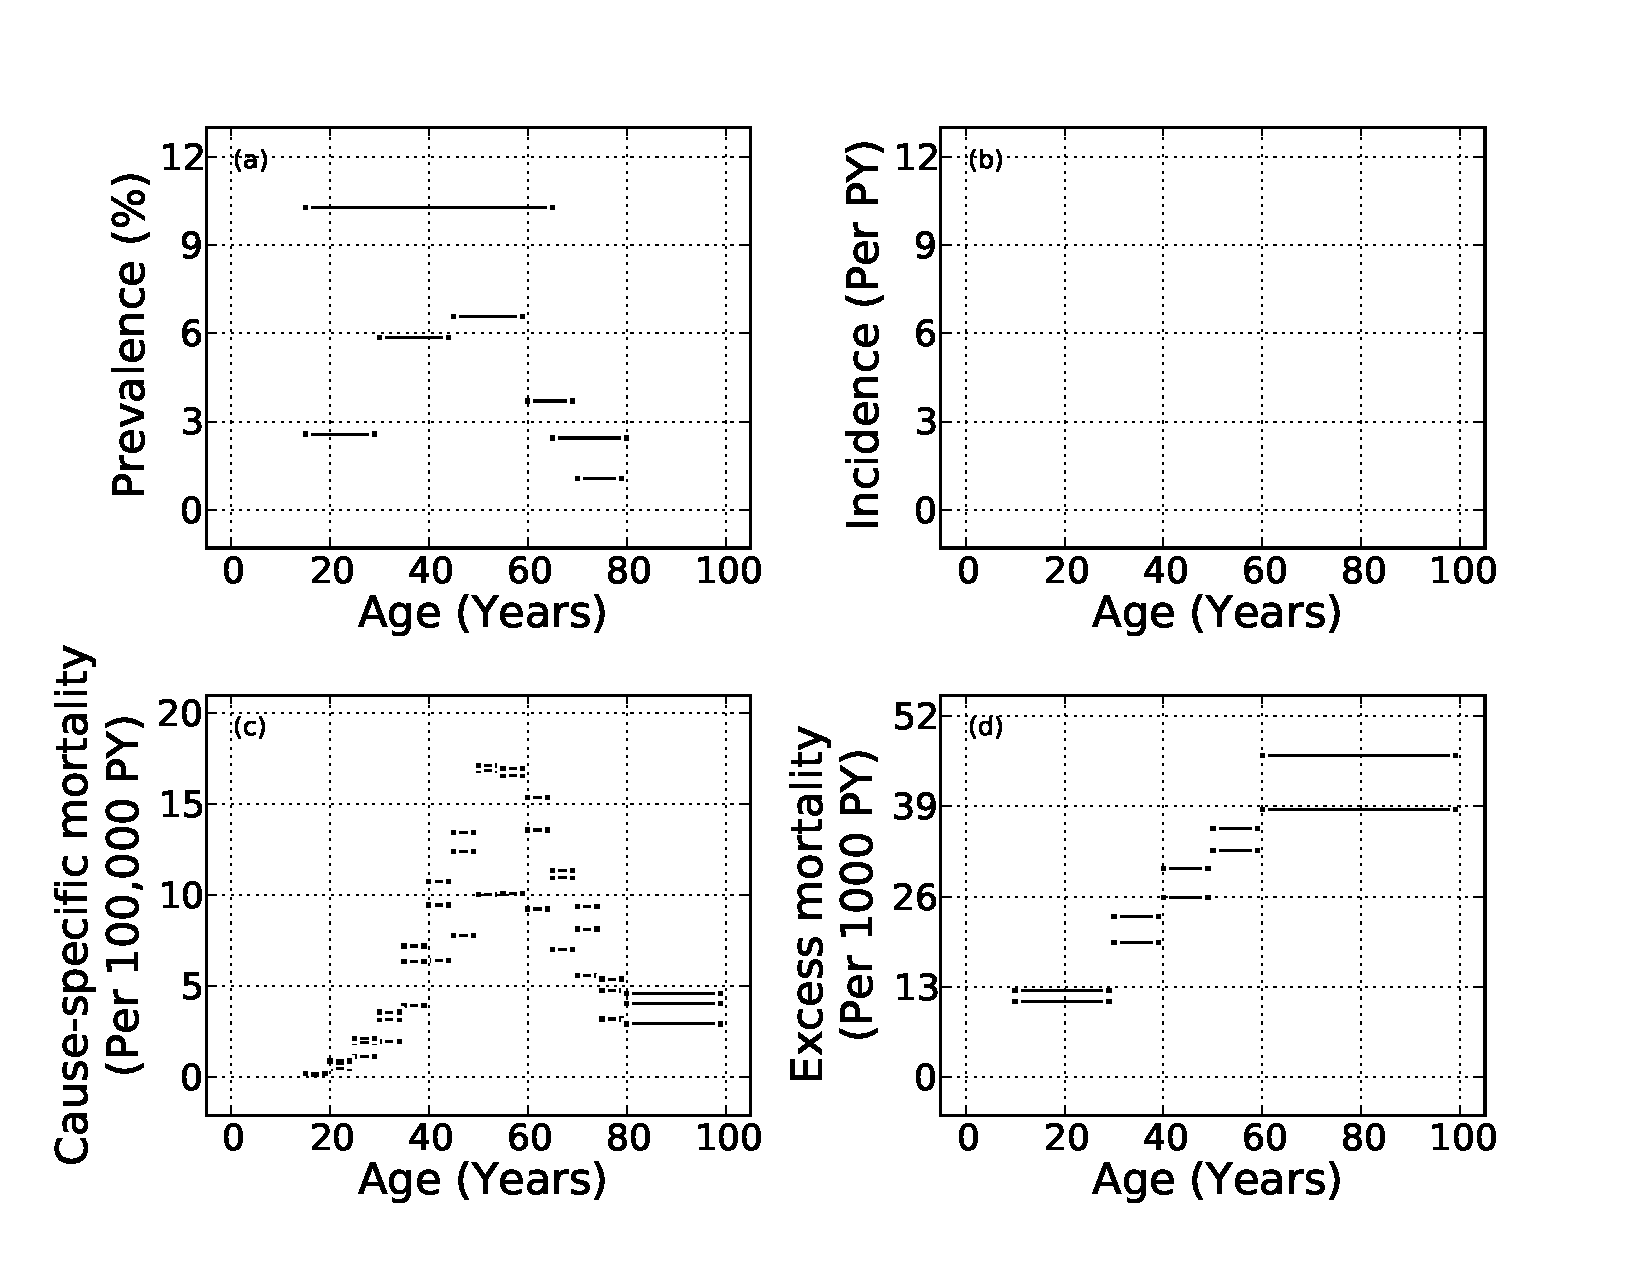
\includegraphics[width=\textwidth]{alcohol-data.pdf}
            \caption{Data on alcohol
              dependence in males from the GBD 2010 Study region of
              Central Asia collected by systematic review for (a) prevalence, (b) incidence, (c)
              cause-specific mortality, and (d) excess mortality.}
            \label{fig:app-alcohol data}
        \end{center}
    \end{figure}

It is important to note that cause-specific mortality in this example
means that the physician issuing a death certificate deemed the person
to have died \emph{of} alcohol dependence and not merely \emph{with} the
condition.  Alcohol dependence likely has a higher excess mortality
than our data suggest for two reasons.  First, alcohol dependence is
a risk factor for other diseases, including stroke and cancers.  In
any individual death from those diseases, it is unlikely that alcohol
dependence was recorded as the underlying cause of
death.\cite{TK_citation_needed} Second, alcohol dependence is
associated with other characteristics that lead to higher mortality
risk, including tobacco smoking and lower socioeconomic
status.\cite{TK_citation_needed}

To include cause-specific mortality data in the compartmental model,
the model in figure~\ref{forward-sim-two-compartment} can be adapted
by splitting the excess mortality $h_{f}$ into two parts (figure
~\ref{fig:two_compartment_2f}): those who die \emph{of} the
condition $h_{f'}$ and those who die \emph{with} the condition but
\emph{not of} it $h_{f''}$.  As described in section
~\ref{theory-csmr}, excess mortality can then be represented as
    \begin{equation*}
        h_{f} = h_{f''} + h_{f'}
    \end{equation*}
While the product of excess mortality and prevalence, $h_{p} \cdot h_{f}$,
can be directly measured, in practice $h_{f''}$ and $h_{f'}$ are never
disentangled.  Our method implicitly separates $h_{f'}$ and $h_{f''}$
but does not try to explicitly represent both.

    \begin{figure}[h]
        \begin{center}
            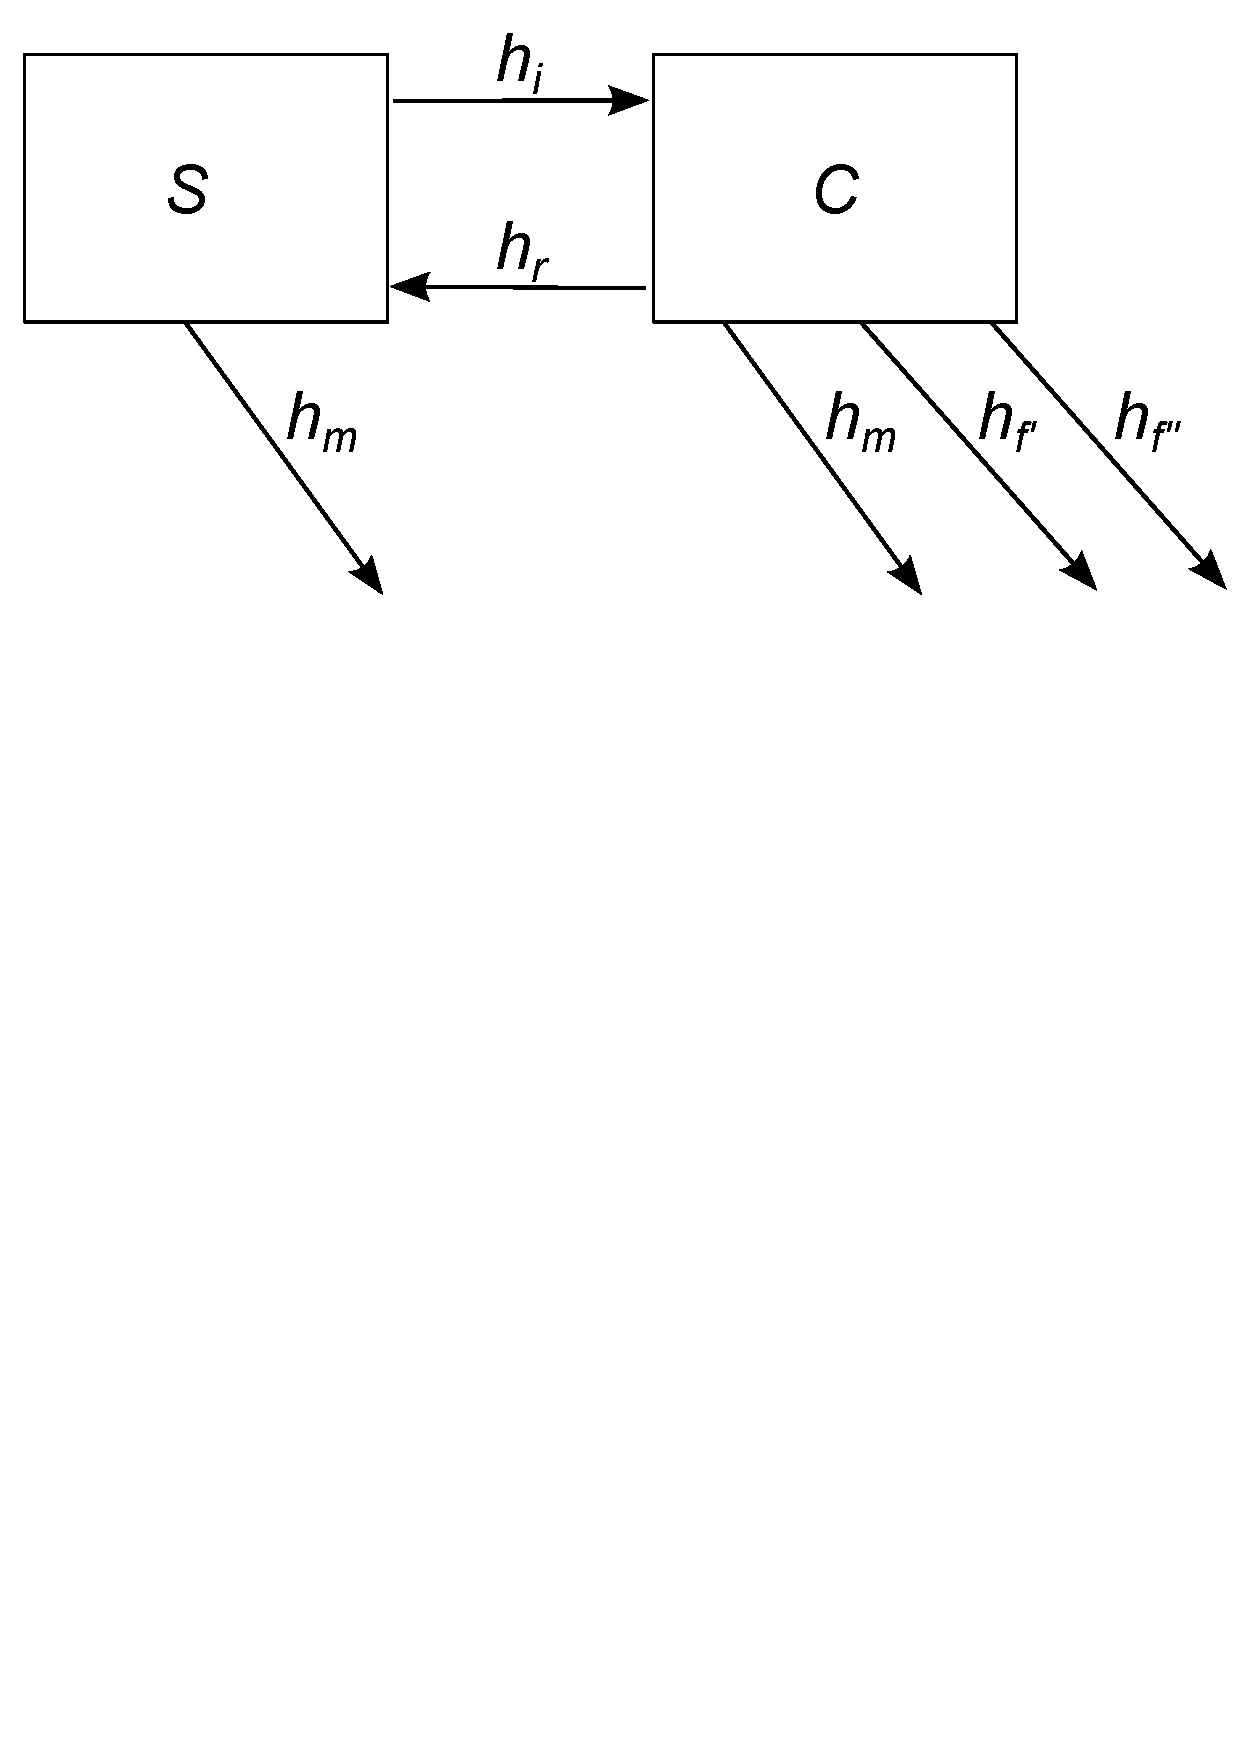
\includegraphics[width=\textwidth]{SC2.pdf}
            \caption{The $2$-compartment mechanistic model with the
              excess mortality split into $2$ hazards.}
            \label{fig:two_compartment_2f}
        \end{center}
    \end{figure}

For some diseases in the GBD 2010 Study, it is a reasonable assumption
that $h_{f''} = 0$, so that those who die with the condition die of
it.  When this is the case, the cause-specific mortality is a direct
estimate of $h_{p} \cdot h_{f}$, a measurement of population
mortality.  However, for diseases such as alcohol dependence, this is
a questionable assumption, for the reasons mentioned above.  When
$h_{f''} \neq 0$, cause-specific mortality data provide the lower
bound on $h_{p} \cdot h_{f}$.

As seen in figure~\ref{fig:app-alcohol compare}, assuming $h_{f''}=0$
instead of $h_{f''}\geq 0$ leads to a change in the estimated prevalence
of the condition.

    \begin{figure}[h]
        \begin{center}
            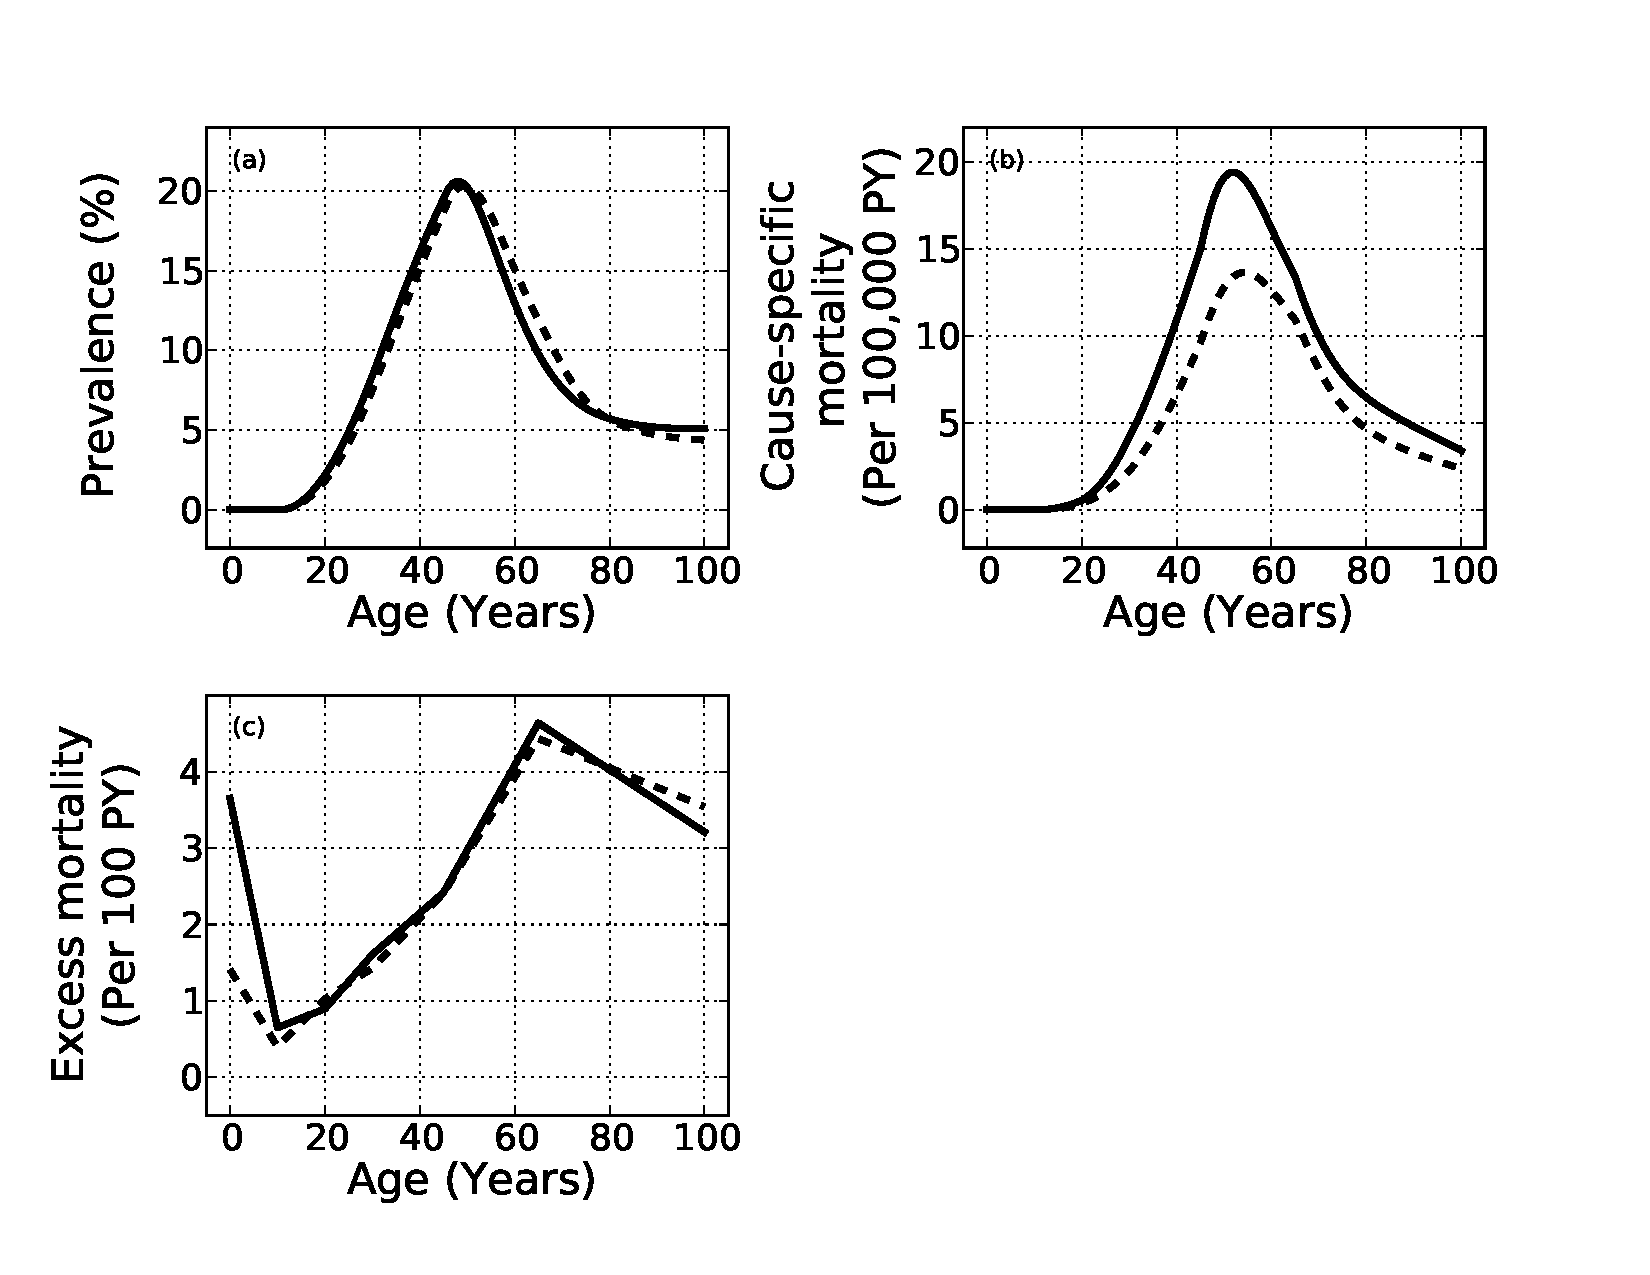
\includegraphics[width=\textwidth]{alcohol-overlay.pdf}
            \caption{Comparison of (a) prevalence,
              (b) cause-specific mortality, and (c) excess
              mortality estimates of alcohol
              dependence in Central Asian males in 2005 when using
              cause-specific mortality data as a lower bound ($h_{f''}$ unrestricted)
              or a direct estimate of the product of
              prevalence and excess mortality ($h_{f''} = 0$).}
            \label{fig:app-alcohol compare}
        \end{center}
    \end{figure}

By decomposing excess mortality into those who die of the
disease and those who die with the disease but not of the disease, the
compartmental model in figure~\ref{forward-sim-two-compartment} can
use the cause-specific mortality data as a lower bound on prevalence
times excess mortality, which is appropriate if the
disease is not exclusively coded as the underlying cause of death.
